\documentclass[twoside]{book}

% Packages required by doxygen
\usepackage{fixltx2e}
\usepackage{calc}
\usepackage{doxygen}
\usepackage[export]{adjustbox} % also loads graphicx
\usepackage{graphicx}
\usepackage[utf8]{inputenc}
\usepackage{makeidx}
\usepackage{multicol}
\usepackage{multirow}
\PassOptionsToPackage{warn}{textcomp}
\usepackage{textcomp}
\usepackage[nointegrals]{wasysym}
\usepackage[table]{xcolor}

% Font selection
\usepackage[T1]{fontenc}
\usepackage[scaled=.90]{helvet}
\usepackage{courier}
\usepackage{amssymb}
\usepackage{sectsty}
\renewcommand{\familydefault}{\sfdefault}
\allsectionsfont{%
  \fontseries{bc}\selectfont%
  \color{darkgray}%
}
\renewcommand{\DoxyLabelFont}{%
  \fontseries{bc}\selectfont%
  \color{darkgray}%
}
\newcommand{\+}{\discretionary{\mbox{\scriptsize$\hookleftarrow$}}{}{}}

% Page & text layout
\usepackage{geometry}
\geometry{%
  a4paper,%
  top=2.5cm,%
  bottom=2.5cm,%
  left=2.5cm,%
  right=2.5cm%
}
\tolerance=750
\hfuzz=15pt
\hbadness=750
\setlength{\emergencystretch}{15pt}
\setlength{\parindent}{0cm}
\setlength{\parskip}{3ex plus 2ex minus 2ex}
\makeatletter
\renewcommand{\paragraph}{%
  \@startsection{paragraph}{4}{0ex}{-1.0ex}{1.0ex}{%
    \normalfont\normalsize\bfseries\SS@parafont%
  }%
}
\renewcommand{\subparagraph}{%
  \@startsection{subparagraph}{5}{0ex}{-1.0ex}{1.0ex}{%
    \normalfont\normalsize\bfseries\SS@subparafont%
  }%
}
\makeatother

% Headers & footers
\usepackage{fancyhdr}
\pagestyle{fancyplain}
\fancyhead[LE]{\fancyplain{}{\bfseries\thepage}}
\fancyhead[CE]{\fancyplain{}{}}
\fancyhead[RE]{\fancyplain{}{\bfseries\leftmark}}
\fancyhead[LO]{\fancyplain{}{\bfseries\rightmark}}
\fancyhead[CO]{\fancyplain{}{}}
\fancyhead[RO]{\fancyplain{}{\bfseries\thepage}}
\fancyfoot[LE]{\fancyplain{}{}}
\fancyfoot[CE]{\fancyplain{}{}}
\fancyfoot[RE]{\fancyplain{}{\bfseries\scriptsize Generated by Doxygen }}
\fancyfoot[LO]{\fancyplain{}{\bfseries\scriptsize Generated by Doxygen }}
\fancyfoot[CO]{\fancyplain{}{}}
\fancyfoot[RO]{\fancyplain{}{}}
\renewcommand{\footrulewidth}{0.4pt}
\renewcommand{\chaptermark}[1]{%
  \markboth{#1}{}%
}
\renewcommand{\sectionmark}[1]{%
  \markright{\thesection\ #1}%
}

% Indices & bibliography
\usepackage{natbib}
\usepackage[titles]{tocloft}
\setcounter{tocdepth}{3}
\setcounter{secnumdepth}{5}
\makeindex

% Hyperlinks (required, but should be loaded last)
\usepackage{ifpdf}
\ifpdf
  \usepackage[pdftex,pagebackref=true]{hyperref}
\else
  \usepackage[ps2pdf,pagebackref=true]{hyperref}
\fi
\hypersetup{%
  colorlinks=true,%
  linkcolor=blue,%
  citecolor=blue,%
  unicode%
}

% Custom commands
\newcommand{\clearemptydoublepage}{%
  \newpage{\pagestyle{empty}\cleardoublepage}%
}

\usepackage{caption}
\captionsetup{labelsep=space,justification=centering,font={bf},singlelinecheck=off,skip=4pt,position=top}

%===== C O N T E N T S =====

\begin{document}

% Titlepage & ToC
\hypersetup{pageanchor=false,
             bookmarksnumbered=true,
             pdfencoding=unicode
            }
\pagenumbering{alph}
\begin{titlepage}
\vspace*{7cm}
\begin{center}%
{\Large My Project }\\
\vspace*{1cm}
{\large Generated by Doxygen 1.8.14}\\
\end{center}
\end{titlepage}
\clearemptydoublepage
\pagenumbering{roman}
\tableofcontents
\clearemptydoublepage
\pagenumbering{arabic}
\hypersetup{pageanchor=true}

%--- Begin generated contents ---
\chapter{Hierarchical Index}
\section{Class Hierarchy}
This inheritance list is sorted roughly, but not completely, alphabetically\+:\begin{DoxyCompactList}
\item \contentsline{section}{pack\+Classes.\+Bone}{\pageref{classpack_classes_1_1_bone}}{}
\item \contentsline{section}{pack\+Classes.\+Finger}{\pageref{classpack_classes_1_1_finger}}{}
\item \contentsline{section}{pack\+Classes.\+Hand}{\pageref{classpack_classes_1_1_hand}}{}
\item \contentsline{section}{pack\+Main.\+Main}{\pageref{classpack_main_1_1_main}}{}
\item \contentsline{section}{pack\+Interface.\+Main\+Frame}{\pageref{classpack_interface_1_1_main_frame}}{}
\item \contentsline{section}{pack\+Digital.\+Serieko\+Linea\+Kontrolatzailea}{\pageref{classpack_digital_1_1_serieko_linea_kontrolatzailea}}{}
\item J\+Frame\begin{DoxyCompactList}
\item \contentsline{section}{pack\+Custom\+Window.\+Pop\+Up}{\pageref{classpack_custom_window_1_1_pop_up}}{}
\begin{DoxyCompactList}
\item \contentsline{section}{pack\+Custom\+Window.\+Pop\+Up\+Tiempo}{\pageref{classpack_custom_window_1_1_pop_up_tiempo}}{}
\end{DoxyCompactList}
\end{DoxyCompactList}
\item J\+Panel\begin{DoxyCompactList}
\item \contentsline{section}{pack\+Interface.\+Animacion\+Texto}{\pageref{classpack_interface_1_1_animacion_texto}}{}
\end{DoxyCompactList}
\item Listener\begin{DoxyCompactList}
\item \contentsline{section}{pack\+Leap\+Motion.\+Gesture\+Controller}{\pageref{classpack_leap_motion_1_1_gesture_controller}}{}
\end{DoxyCompactList}
\end{DoxyCompactList}

\chapter{Class Index}
\section{Class List}
Here are the classes, structs, unions and interfaces with brief descriptions\+:\begin{DoxyCompactList}
\item\contentsline{section}{\mbox{\hyperlink{classpack_interface_1_1_animacion_texto}{pack\+Interface.\+Animacion\+Texto}} }{\pageref{classpack_interface_1_1_animacion_texto}}{}
\item\contentsline{section}{\mbox{\hyperlink{classpack_classes_1_1_bone}{pack\+Classes.\+Bone}} }{\pageref{classpack_classes_1_1_bone}}{}
\item\contentsline{section}{\mbox{\hyperlink{classpack_classes_1_1_finger}{pack\+Classes.\+Finger}} }{\pageref{classpack_classes_1_1_finger}}{}
\item\contentsline{section}{\mbox{\hyperlink{classpack_leap_motion_1_1_gesture_controller}{pack\+Leap\+Motion.\+Gesture\+Controller}} }{\pageref{classpack_leap_motion_1_1_gesture_controller}}{}
\item\contentsline{section}{\mbox{\hyperlink{classpack_classes_1_1_hand}{pack\+Classes.\+Hand}} }{\pageref{classpack_classes_1_1_hand}}{}
\item\contentsline{section}{\mbox{\hyperlink{classpack_main_1_1_main}{pack\+Main.\+Main}} }{\pageref{classpack_main_1_1_main}}{}
\item\contentsline{section}{\mbox{\hyperlink{classpack_interface_1_1_main_frame}{pack\+Interface.\+Main\+Frame}} }{\pageref{classpack_interface_1_1_main_frame}}{}
\item\contentsline{section}{\mbox{\hyperlink{classpack_custom_window_1_1_pop_up}{pack\+Custom\+Window.\+Pop\+Up}} }{\pageref{classpack_custom_window_1_1_pop_up}}{}
\item\contentsline{section}{\mbox{\hyperlink{classpack_custom_window_1_1_pop_up_tiempo}{pack\+Custom\+Window.\+Pop\+Up\+Tiempo}} }{\pageref{classpack_custom_window_1_1_pop_up_tiempo}}{}
\item\contentsline{section}{\mbox{\hyperlink{classpack_digital_1_1_serieko_linea_kontrolatzailea}{pack\+Digital.\+Serieko\+Linea\+Kontrolatzailea}} }{\pageref{classpack_digital_1_1_serieko_linea_kontrolatzailea}}{}
\end{DoxyCompactList}

\chapter{Class Documentation}
\hypertarget{classpack_interface_1_1_animacion_texto}{}\section{pack\+Interface.\+Animacion\+Texto Class Reference}
\label{classpack_interface_1_1_animacion_texto}\index{pack\+Interface.\+Animacion\+Texto@{pack\+Interface.\+Animacion\+Texto}}


Inheritance diagram for pack\+Interface.\+Animacion\+Texto\+:
\nopagebreak
\begin{figure}[H]
\begin{center}
\leavevmode
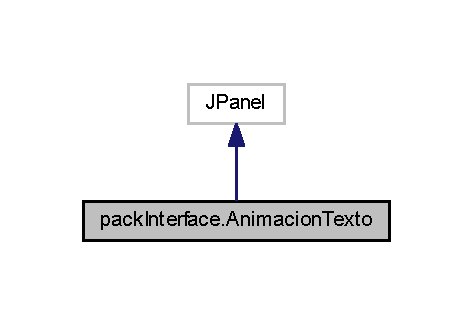
\includegraphics[width=227pt]{classpack_interface_1_1_animacion_texto__inherit__graph}
\end{center}
\end{figure}


Collaboration diagram for pack\+Interface.\+Animacion\+Texto\+:
\nopagebreak
\begin{figure}[H]
\begin{center}
\leavevmode
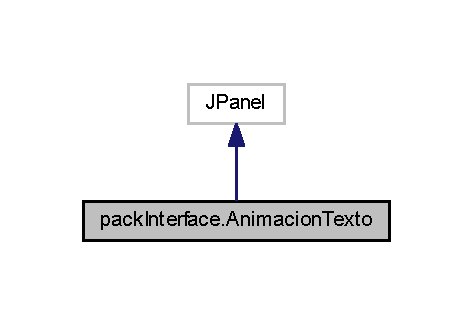
\includegraphics[width=227pt]{classpack_interface_1_1_animacion_texto__coll__graph}
\end{center}
\end{figure}
\subsection*{Public Member Functions}
\begin{DoxyCompactItemize}
\item 
\mbox{\hyperlink{classpack_interface_1_1_animacion_texto_ab74997ca3cbe6518ac17daed9dcd2b77}{Animacion\+Texto}} ()
\item 
\mbox{\Hypertarget{classpack_interface_1_1_animacion_texto_ae9c7a461fb1291082b1b6fd9674a4849}\label{classpack_interface_1_1_animacion_texto_ae9c7a461fb1291082b1b6fd9674a4849}} 
void {\bfseries paint} (Graphics g)
\item 
\mbox{\Hypertarget{classpack_interface_1_1_animacion_texto_a3ebfa5522b2f4337870f8cda791d9c21}\label{classpack_interface_1_1_animacion_texto_a3ebfa5522b2f4337870f8cda791d9c21}} 
void {\bfseries start} ()
\end{DoxyCompactItemize}


\subsection{Constructor \& Destructor Documentation}
\mbox{\Hypertarget{classpack_interface_1_1_animacion_texto_ab74997ca3cbe6518ac17daed9dcd2b77}\label{classpack_interface_1_1_animacion_texto_ab74997ca3cbe6518ac17daed9dcd2b77}} 
\index{pack\+Interface\+::\+Animacion\+Texto@{pack\+Interface\+::\+Animacion\+Texto}!Animacion\+Texto@{Animacion\+Texto}}
\index{Animacion\+Texto@{Animacion\+Texto}!pack\+Interface\+::\+Animacion\+Texto@{pack\+Interface\+::\+Animacion\+Texto}}
\subsubsection{\texorpdfstring{Animacion\+Texto()}{AnimacionTexto()}}
{\footnotesize\ttfamily pack\+Interface.\+Animacion\+Texto.\+Animacion\+Texto (\begin{DoxyParamCaption}{ }\end{DoxyParamCaption})}


\begin{DoxyParams}{Parameters}
{\em args} & \\
\hline
\end{DoxyParams}


The documentation for this class was generated from the following file\+:\begin{DoxyCompactItemize}
\item 
C\+:/\+Users/\+Ander/\+Documents/\+Java/\+Proyecto\+Casa\+Domotica/src/pack\+Interface/Animacion\+Texto.\+java\end{DoxyCompactItemize}

\hypertarget{classpack_classes_1_1_bone}{}\section{pack\+Classes.\+Bone Class Reference}
\label{classpack_classes_1_1_bone}\index{pack\+Classes.\+Bone@{pack\+Classes.\+Bone}}
\subsection*{Public Member Functions}
\begin{DoxyCompactItemize}
\item 
\mbox{\Hypertarget{classpack_classes_1_1_bone_a309f8b47e609a32b4ff5684833e21b89}\label{classpack_classes_1_1_bone_a309f8b47e609a32b4ff5684833e21b89}} 
{\bfseries Bone} (float x, float y, float z, boolean is\+Hand)
\item 
\mbox{\Hypertarget{classpack_classes_1_1_bone_aa97b6423202ae70d611e6e543b551abb}\label{classpack_classes_1_1_bone_aa97b6423202ae70d611e6e543b551abb}} 
float {\bfseries get\+PosX} ()
\item 
\mbox{\Hypertarget{classpack_classes_1_1_bone_a0ef091c057fd11820b64e8f5a5a165e9}\label{classpack_classes_1_1_bone_a0ef091c057fd11820b64e8f5a5a165e9}} 
float {\bfseries get\+PosY} ()
\item 
\mbox{\Hypertarget{classpack_classes_1_1_bone_aa124e5b4a00e34b38d90cc1e044165f3}\label{classpack_classes_1_1_bone_aa124e5b4a00e34b38d90cc1e044165f3}} 
float {\bfseries get\+PosZ} ()
\end{DoxyCompactItemize}


The documentation for this class was generated from the following file\+:\begin{DoxyCompactItemize}
\item 
C\+:/\+Users/\+Ander/\+Documents/\+Java/\+Proyecto\+Casa\+Domotica/src/pack\+Classes/Bone.\+java\end{DoxyCompactItemize}

\hypertarget{classpack_classes_1_1_finger}{}\section{pack\+Classes.\+Finger Class Reference}
\label{classpack_classes_1_1_finger}\index{pack\+Classes.\+Finger@{pack\+Classes.\+Finger}}
\subsection*{Public Member Functions}
\begin{DoxyCompactItemize}
\item 
\mbox{\Hypertarget{classpack_classes_1_1_finger_a99a982d6c6908fe5aed6a58cead7f2b0}\label{classpack_classes_1_1_finger_a99a982d6c6908fe5aed6a58cead7f2b0}} 
void {\bfseries add\+Element} (\mbox{\hyperlink{classpack_classes_1_1_bone}{Bone}} e)
\item 
\mbox{\Hypertarget{classpack_classes_1_1_finger_ab5d153c2d94417280430f0ee6025b1bf}\label{classpack_classes_1_1_finger_ab5d153c2d94417280430f0ee6025b1bf}} 
Array\+List$<$ \mbox{\hyperlink{classpack_classes_1_1_bone}{Bone}} $>$ {\bfseries get\+Bones} ()
\item 
\mbox{\Hypertarget{classpack_classes_1_1_finger_a80ea0752803fbf7c423acc124fc5770d}\label{classpack_classes_1_1_finger_a80ea0752803fbf7c423acc124fc5770d}} 
Array\+List$<$ \mbox{\hyperlink{classpack_classes_1_1_bone}{Bone}} $>$ {\bfseries get\+List} ()
\end{DoxyCompactItemize}


The documentation for this class was generated from the following file\+:\begin{DoxyCompactItemize}
\item 
C\+:/\+Users/\+Ander/\+Documents/\+Java/\+Proyecto\+Casa\+Domotica/src/pack\+Classes/Finger.\+java\end{DoxyCompactItemize}

\hypertarget{classpack_leap_motion_1_1_gesture_controller}{}\section{pack\+Leap\+Motion.\+Gesture\+Controller Class Reference}
\label{classpack_leap_motion_1_1_gesture_controller}\index{pack\+Leap\+Motion.\+Gesture\+Controller@{pack\+Leap\+Motion.\+Gesture\+Controller}}


Inheritance diagram for pack\+Leap\+Motion.\+Gesture\+Controller\+:
\nopagebreak
\begin{figure}[H]
\begin{center}
\leavevmode
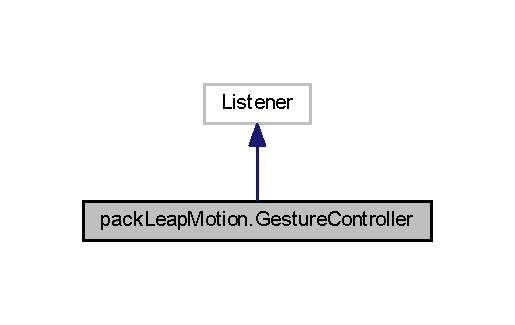
\includegraphics[width=247pt]{classpack_leap_motion_1_1_gesture_controller__inherit__graph}
\end{center}
\end{figure}


Collaboration diagram for pack\+Leap\+Motion.\+Gesture\+Controller\+:
\nopagebreak
\begin{figure}[H]
\begin{center}
\leavevmode
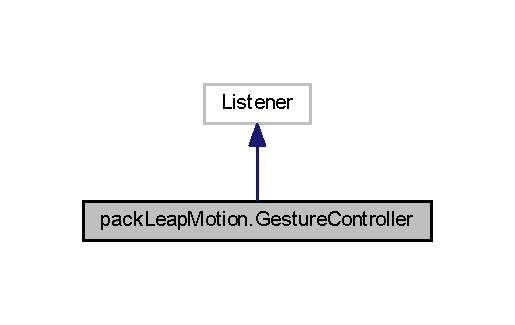
\includegraphics[width=247pt]{classpack_leap_motion_1_1_gesture_controller__coll__graph}
\end{center}
\end{figure}
\subsection*{Public Member Functions}
\begin{DoxyCompactItemize}
\item 
\mbox{\Hypertarget{classpack_leap_motion_1_1_gesture_controller_a8315f6be678b327266d0c3926ce26133}\label{classpack_leap_motion_1_1_gesture_controller_a8315f6be678b327266d0c3926ce26133}} 
{\bfseries Gesture\+Controller} (\mbox{\hyperlink{classpack_interface_1_1_main_frame}{Main\+Frame}} window)
\item 
\mbox{\Hypertarget{classpack_leap_motion_1_1_gesture_controller_a9998ec8be3ea657d06cf775c02388d9f}\label{classpack_leap_motion_1_1_gesture_controller_a9998ec8be3ea657d06cf775c02388d9f}} 
void {\bfseries on\+Connect} (Controller controller)
\item 
\mbox{\Hypertarget{classpack_leap_motion_1_1_gesture_controller_a1cdf76d24a13ff0a90aad04325c9453b}\label{classpack_leap_motion_1_1_gesture_controller_a1cdf76d24a13ff0a90aad04325c9453b}} 
void {\bfseries on\+Disconnect} (Controller controller)
\item 
\mbox{\Hypertarget{classpack_leap_motion_1_1_gesture_controller_aea88530c7a99ed756b4aa46bf290a950}\label{classpack_leap_motion_1_1_gesture_controller_aea88530c7a99ed756b4aa46bf290a950}} 
void {\bfseries on\+Frame} (Controller controller)
\item 
\mbox{\Hypertarget{classpack_leap_motion_1_1_gesture_controller_a5d5126bf0481a7dd37fa411b0b7382a5}\label{classpack_leap_motion_1_1_gesture_controller_a5d5126bf0481a7dd37fa411b0b7382a5}} 
boolean {\bfseries has\+Hand} (Frame frame)
\end{DoxyCompactItemize}


The documentation for this class was generated from the following file\+:\begin{DoxyCompactItemize}
\item 
C\+:/\+Users/\+Ander/\+Documents/\+Java/\+Proyecto\+Casa\+Domotica/src/pack\+Leap\+Motion/Gesture\+Controller.\+java\end{DoxyCompactItemize}

\hypertarget{classpack_classes_1_1_hand}{}\section{pack\+Classes.\+Hand Class Reference}
\label{classpack_classes_1_1_hand}\index{pack\+Classes.\+Hand@{pack\+Classes.\+Hand}}


Collaboration diagram for pack\+Classes.\+Hand\+:
\nopagebreak
\begin{figure}[H]
\begin{center}
\leavevmode
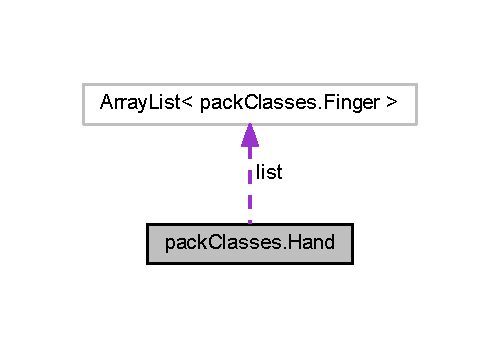
\includegraphics[width=240pt]{classpack_classes_1_1_hand__coll__graph}
\end{center}
\end{figure}
\subsection*{Public Member Functions}
\begin{DoxyCompactItemize}
\item 
\mbox{\Hypertarget{classpack_classes_1_1_hand_a242c41d0a17f6b215263482594ae3c51}\label{classpack_classes_1_1_hand_a242c41d0a17f6b215263482594ae3c51}} 
{\bfseries Hand} (float x, float y, float z)
\item 
\mbox{\Hypertarget{classpack_classes_1_1_hand_ac9c9bbef53fd8cacef78faff64a7a66d}\label{classpack_classes_1_1_hand_ac9c9bbef53fd8cacef78faff64a7a66d}} 
void {\bfseries add\+Finger} (\mbox{\hyperlink{classpack_classes_1_1_finger}{Finger}} e)
\item 
\mbox{\Hypertarget{classpack_classes_1_1_hand_a1d7ef1e6baa7529538124e4f02b5363e}\label{classpack_classes_1_1_hand_a1d7ef1e6baa7529538124e4f02b5363e}} 
Array\+List$<$ \mbox{\hyperlink{classpack_classes_1_1_finger}{Finger}} $>$ {\bfseries get\+List} ()
\item 
\mbox{\Hypertarget{classpack_classes_1_1_hand_a745ce995b2a86f52e1618ba1e417c972}\label{classpack_classes_1_1_hand_a745ce995b2a86f52e1618ba1e417c972}} 
float {\bfseries get\+PosX} ()
\item 
\mbox{\Hypertarget{classpack_classes_1_1_hand_a363461f4e710bc9c5311247ce1ade6d0}\label{classpack_classes_1_1_hand_a363461f4e710bc9c5311247ce1ade6d0}} 
float {\bfseries get\+PosY} ()
\item 
\mbox{\Hypertarget{classpack_classes_1_1_hand_a460322f622a81e96c6139e1bf1e95cb9}\label{classpack_classes_1_1_hand_a460322f622a81e96c6139e1bf1e95cb9}} 
float {\bfseries get\+PosZ} ()
\item 
\mbox{\Hypertarget{classpack_classes_1_1_hand_afa2f75f64c8049a207f8d6aa4c05af36}\label{classpack_classes_1_1_hand_afa2f75f64c8049a207f8d6aa4c05af36}} 
void {\bfseries show\+Hand} ()
\end{DoxyCompactItemize}


The documentation for this class was generated from the following file\+:\begin{DoxyCompactItemize}
\item 
C\+:/\+Users/\+Ander/\+Documents/\+Java/\+Proyecto\+Casa\+Domotica/src/pack\+Classes/Hand.\+java\end{DoxyCompactItemize}

\hypertarget{classpack_main_1_1_main}{}\section{pack\+Main.\+Main Class Reference}
\label{classpack_main_1_1_main}\index{pack\+Main.\+Main@{pack\+Main.\+Main}}
\subsection*{Static Public Member Functions}
\begin{DoxyCompactItemize}
\item 
\mbox{\Hypertarget{classpack_main_1_1_main_a9f56025f10849a4cd4b6566e781e361a}\label{classpack_main_1_1_main_a9f56025f10849a4cd4b6566e781e361a}} 
static void {\bfseries main} (String\mbox{[}$\,$\mbox{]} args)
\end{DoxyCompactItemize}


The documentation for this class was generated from the following file\+:\begin{DoxyCompactItemize}
\item 
C\+:/\+Users/\+Ander/\+Documents/\+Java/\+Proyecto\+Casa\+Domotica/src/pack\+Main/Main.\+java\end{DoxyCompactItemize}

\hypertarget{classpack_interface_1_1_main_frame}{}\section{pack\+Interface.\+Main\+Frame Class Reference}
\label{classpack_interface_1_1_main_frame}\index{pack\+Interface.\+Main\+Frame@{pack\+Interface.\+Main\+Frame}}


Collaboration diagram for pack\+Interface.\+Main\+Frame\+:
\nopagebreak
\begin{figure}[H]
\begin{center}
\leavevmode
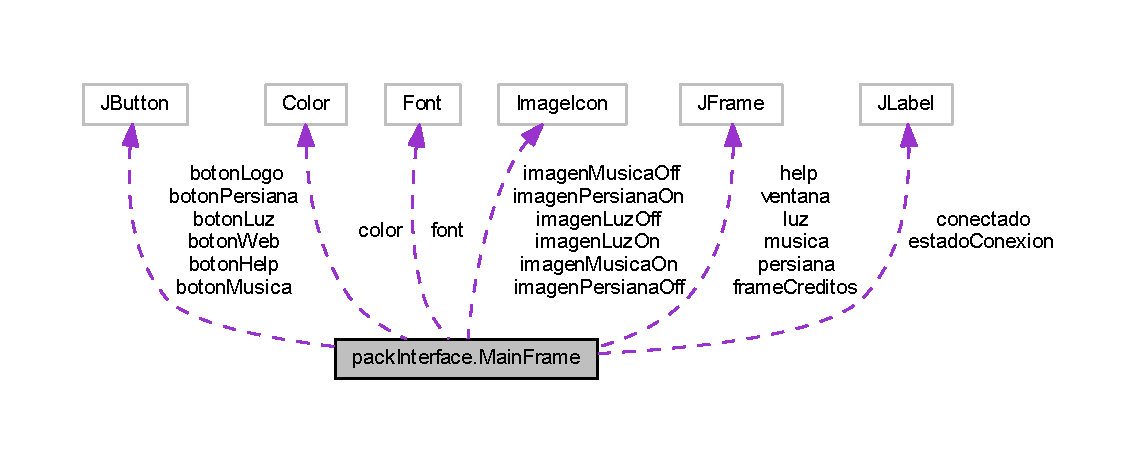
\includegraphics[width=350pt]{classpack_interface_1_1_main_frame__coll__graph}
\end{center}
\end{figure}
\subsection*{Public Member Functions}
\begin{DoxyCompactItemize}
\item 
\mbox{\Hypertarget{classpack_interface_1_1_main_frame_a4201e4a79d5b48a8cc3b72baf74d719e}\label{classpack_interface_1_1_main_frame_a4201e4a79d5b48a8cc3b72baf74d719e}} 
void {\bfseries toggle\+Lights} ()
\item 
\mbox{\Hypertarget{classpack_interface_1_1_main_frame_a7b194ecb7dafadd0728ecf81bcc6056d}\label{classpack_interface_1_1_main_frame_a7b194ecb7dafadd0728ecf81bcc6056d}} 
void {\bfseries toggle\+Persiana} ()
\item 
\mbox{\Hypertarget{classpack_interface_1_1_main_frame_a90d3cc9d32aa54e8401a9c28f938db26}\label{classpack_interface_1_1_main_frame_a90d3cc9d32aa54e8401a9c28f938db26}} 
void {\bfseries toggle\+Music} ()
\item 
\mbox{\Hypertarget{classpack_interface_1_1_main_frame_a2c1b89055920c04cdcf61c2be598ee1c}\label{classpack_interface_1_1_main_frame_a2c1b89055920c04cdcf61c2be598ee1c}} 
void {\bfseries conexion} (boolean estado)
\end{DoxyCompactItemize}
\subsection*{Static Public Member Functions}
\begin{DoxyCompactItemize}
\item 
\mbox{\Hypertarget{classpack_interface_1_1_main_frame_a0540256548b21e4573e070db23bdce88}\label{classpack_interface_1_1_main_frame_a0540256548b21e4573e070db23bdce88}} 
static void {\bfseries Cierra\+Creditos} ()
\end{DoxyCompactItemize}
\subsection*{Protected Member Functions}
\begin{DoxyCompactItemize}
\item 
\mbox{\Hypertarget{classpack_interface_1_1_main_frame_aa90e27d66e1f9e3eaae6a79d81f34b61}\label{classpack_interface_1_1_main_frame_aa90e27d66e1f9e3eaae6a79d81f34b61}} 
void {\bfseries abrir\+Web} ()
\end{DoxyCompactItemize}


The documentation for this class was generated from the following file\+:\begin{DoxyCompactItemize}
\item 
C\+:/\+Users/\+Ander/\+Documents/\+Java/\+Proyecto\+Casa\+Domotica/src/pack\+Interface/Main\+Frame.\+java\end{DoxyCompactItemize}

\hypertarget{classpack_custom_window_1_1_pop_up}{}\section{pack\+Custom\+Window.\+Pop\+Up Class Reference}
\label{classpack_custom_window_1_1_pop_up}\index{pack\+Custom\+Window.\+Pop\+Up@{pack\+Custom\+Window.\+Pop\+Up}}


Inheritance diagram for pack\+Custom\+Window.\+Pop\+Up\+:
\nopagebreak
\begin{figure}[H]
\begin{center}
\leavevmode
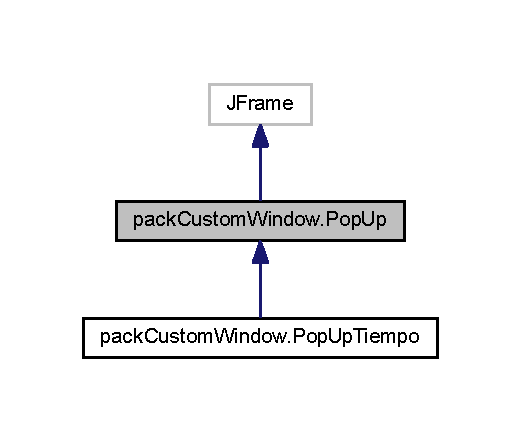
\includegraphics[width=250pt]{classpack_custom_window_1_1_pop_up__inherit__graph}
\end{center}
\end{figure}


Collaboration diagram for pack\+Custom\+Window.\+Pop\+Up\+:
\nopagebreak
\begin{figure}[H]
\begin{center}
\leavevmode
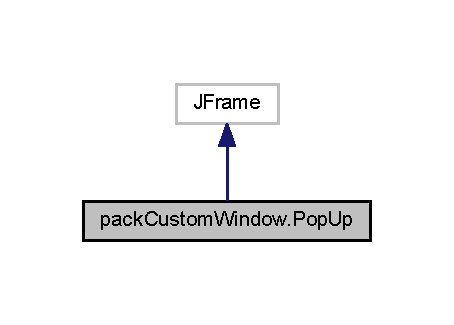
\includegraphics[width=218pt]{classpack_custom_window_1_1_pop_up__coll__graph}
\end{center}
\end{figure}
\subsection*{Public Member Functions}
\begin{DoxyCompactItemize}
\item 
\mbox{\Hypertarget{classpack_custom_window_1_1_pop_up_ac1f51f735e63bc5f33dbe17e82cc3e89}\label{classpack_custom_window_1_1_pop_up_ac1f51f735e63bc5f33dbe17e82cc3e89}} 
{\bfseries Pop\+Up} (String p\+Title\+Name, String p\+Gif\+Name)
\end{DoxyCompactItemize}


The documentation for this class was generated from the following file\+:\begin{DoxyCompactItemize}
\item 
C\+:/\+Users/\+Ander/\+Documents/\+Java/\+Proyecto\+Casa\+Domotica/src/pack\+Custom\+Window/Pop\+Up.\+java\end{DoxyCompactItemize}

\hypertarget{classpack_custom_window_1_1_pop_up_tiempo}{}\section{pack\+Custom\+Window.\+Pop\+Up\+Tiempo Class Reference}
\label{classpack_custom_window_1_1_pop_up_tiempo}\index{pack\+Custom\+Window.\+Pop\+Up\+Tiempo@{pack\+Custom\+Window.\+Pop\+Up\+Tiempo}}


Inheritance diagram for pack\+Custom\+Window.\+Pop\+Up\+Tiempo\+:
\nopagebreak
\begin{figure}[H]
\begin{center}
\leavevmode
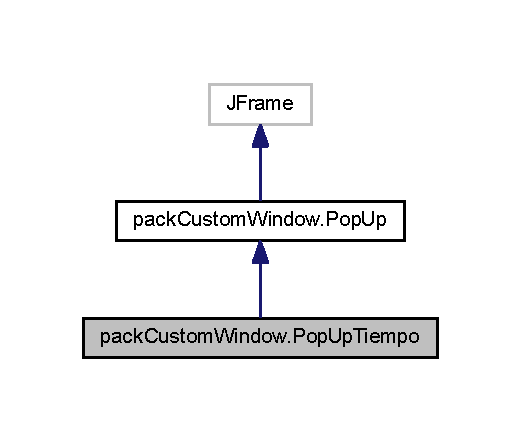
\includegraphics[width=250pt]{classpack_custom_window_1_1_pop_up_tiempo__inherit__graph}
\end{center}
\end{figure}


Collaboration diagram for pack\+Custom\+Window.\+Pop\+Up\+Tiempo\+:
\nopagebreak
\begin{figure}[H]
\begin{center}
\leavevmode
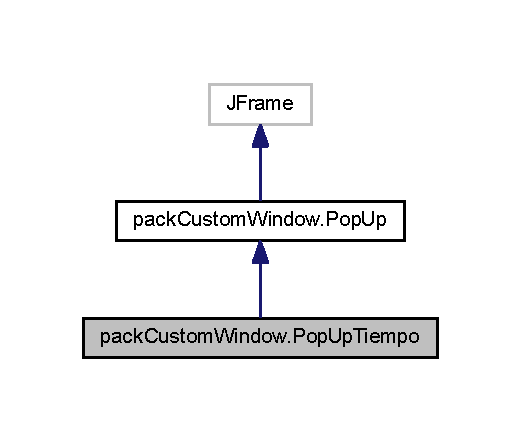
\includegraphics[width=250pt]{classpack_custom_window_1_1_pop_up_tiempo__coll__graph}
\end{center}
\end{figure}
\subsection*{Public Member Functions}
\begin{DoxyCompactItemize}
\item 
\mbox{\Hypertarget{classpack_custom_window_1_1_pop_up_tiempo_a7cc512d6d1807b3c1ad1eb3e1e6c9eac}\label{classpack_custom_window_1_1_pop_up_tiempo_a7cc512d6d1807b3c1ad1eb3e1e6c9eac}} 
{\bfseries Pop\+Up\+Tiempo} (String p\+Title\+Name, String p\+Gif\+Name, int p\+Time)
\end{DoxyCompactItemize}


The documentation for this class was generated from the following file\+:\begin{DoxyCompactItemize}
\item 
C\+:/\+Users/\+Ander/\+Documents/\+Java/\+Proyecto\+Casa\+Domotica/src/pack\+Custom\+Window/Pop\+Up\+Tiempo.\+java\end{DoxyCompactItemize}

\hypertarget{classpack_digital_1_1_serieko_linea_kontrolatzailea}{}\section{pack\+Digital.\+Serieko\+Linea\+Kontrolatzailea Class Reference}
\label{classpack_digital_1_1_serieko_linea_kontrolatzailea}\index{pack\+Digital.\+Serieko\+Linea\+Kontrolatzailea@{pack\+Digital.\+Serieko\+Linea\+Kontrolatzailea}}
\subsection*{Public Member Functions}
\begin{DoxyCompactItemize}
\item 
\mbox{\Hypertarget{classpack_digital_1_1_serieko_linea_kontrolatzailea_a135049670b4a187f99928bbe417d4990}\label{classpack_digital_1_1_serieko_linea_kontrolatzailea_a135049670b4a187f99928bbe417d4990}} 
{\bfseries Serieko\+Linea\+Kontrolatzailea} (J\+Frame ventana)
\item 
\mbox{\Hypertarget{classpack_digital_1_1_serieko_linea_kontrolatzailea_a8cf08ea2dfe583f095c4d2d2eb069af2}\label{classpack_digital_1_1_serieko_linea_kontrolatzailea_a8cf08ea2dfe583f095c4d2d2eb069af2}} 
int {\bfseries leer\+Contrase�a} ()  throws I\+O\+Exception
\item 
\mbox{\Hypertarget{classpack_digital_1_1_serieko_linea_kontrolatzailea_a15741752ff8a867595ed01ce6d77fc6d}\label{classpack_digital_1_1_serieko_linea_kontrolatzailea_a15741752ff8a867595ed01ce6d77fc6d}} 
void {\bfseries close} ()
\end{DoxyCompactItemize}


The documentation for this class was generated from the following file\+:\begin{DoxyCompactItemize}
\item 
C\+:/\+Users/\+Ander/\+Documents/\+Java/\+Proyecto\+Casa\+Domotica/src/pack\+Digital/Serieko\+Linea\+Kontrolatzailea.\+java\end{DoxyCompactItemize}

%--- End generated contents ---

% Index
\backmatter
\newpage
\phantomsection
\clearemptydoublepage
\addcontentsline{toc}{chapter}{Index}
\printindex

\end{document}
